\section{Maintain: trainable repair under a certified budget}
\label{sec:maintain}

Certification (\S\ref{sec:certify}) tells us \emph{whether} a store is still valid; it does not by itself make maintenance better. This section asks two questions: can the maintainer that rewrites pages under new documents be improved beyond prompting, and can we bound the damage a maintainer causes \emph{as it happens}, rather than only measuring it after the fact.

\subsection{A trained maintainer beats the best prompt, honestly scored}

We compare a minimal offline best-of-$k$ SFT-trained maintainer against the strongest prompted maintainer (\texttt{anchored}) and a vanilla baseline, all at equal deploy cost (single forward pass per rewrite; the SFT cost is paid once, offline). On a $12$-round rewrite protocol ($5$ seeds each), the trained maintainer reaches $R_{12} = 0.523 \pm 0.037$ vs.\ the anchored prompt's $0.397 \pm 0.059$ --- a gain of $+0.127$ (bootstrap $95\%$ CI $[0.067, 0.187]$, Welch $p{=}0.009$) --- against a vanilla baseline of $0.278 \pm 0.052$ and a fresh-rebuild ceiling of $0.552 \pm 0.036$ ($n{=}19$). The trained maintainer recovers $90\%$ of the maintained-vs-rebuild gap, vs.\ $43\%$ (anchored) and $47\%$ (a second, conservative prompt).

We deliberately do \emph{not} claim this result is Pareto-optimal across retention and incorporation (the rate at which new information is successfully written in): the incorporation gain of the trained maintainer over anchored ($0.088$ vs.\ $0.083$) is statistically null (Welch $p{=}0.54$). The honest claim is narrower and still useful: the trained maintainer dominates on retention at incorporation no lower than the prompt's --- not a two-dimensional Pareto win.

\paragraph{A budget-gated boundary for reward gaming.} Offline best-of-$k$ selection could in principle be gamed --- optimizing for whatever proxy signal selects the training data, rather than true fidelity. We measure this directly: the gap between the selection \emph{signal}'s and the resulting \emph{policy}'s gameability rises with how binding the page-length budget is. At a slack budget ($350$ words), the signal-level gameable gap is $0.048$--$0.062$ and the distilled policy's difference-in-differences stays $\approx 0$ ($-0.010$ to $+0.009$); at a binding budget ($120$ words), the signal gap rises to $0.127$--$0.136$ ($\sim\!2.5\times$) while the policy DiD rises only to $0.020$--$0.024$ --- offline distillation ``launders'' roughly $6\times$ of the gameable signal out. We flag two honest weaknesses in this result: the binding-budget policy DiD ($+0.022$) sits below its own estimated binomial noise floor ($\sim 0.038$), so the quantitative $6\times$ figure is a ratio of two small, noisy quantities that could plausibly range from $3\times$ to unbounded; and the \emph{dangerous} half of this boundary law --- what happens under an RL-trained maintainer or a fixed, predictable audit schedule, where gaming the signal is directly the training objective rather than a side effect of selection --- has not been run. We name this as the single largest open risk in the maintenance stage, not as a solved case.

\subsection{LossGate: a per-batch, anytime-valid retention bound}

The trained maintainer above still loses information; \S\ref{sec:certify}'s certificate tells us afterward how much. LossGate instead wraps \emph{any} maintainer (prompted, trained, or otherwise) with a gate-and-rollback wrapper that emits, every batch $t$, a certified worst-case bound $R(t) \ge R(t-1) - b_t$ at confidence $1-\delta$, where $b_t$ is a judge-noise-corrected Clopper-Pearson upper bound on the fraction of previously-confirmed facts destroyed that batch, estimated on a held-out probe pool the maintainer never sees. Per-batch bounds are composed across the full stream via Basel-weighted significance levels ($\alpha_t = \delta \cdot 6/(\pi^2 t^2)$, $\sum_t \alpha_t \le \delta$) into a single \emph{anytime-valid} stream bound $R(t) \ge L_0 - \sum_{s \le t} b_t[s]$ that holds simultaneously at every $t$ with no fixed horizon --- a confidence-sequence guarantee, not a bound computed for one chosen stopping time.

\begin{table}[h]
\centering
\small
\caption{LossGate, 7-seed final numbers. $R(12)$ is retention after 12 batches; paired gain is the per-seed difference between the gated and ungated version of the same maintainer.}
\label{tab:lossgate}
\begin{tabular}{lcc}
\toprule
Maintainer & $R(12)$, ungated & $R(12)$, LossGate-wrapped \\
\midrule
Vanilla prompt & $0.285 \pm 0.05$ & $0.405 \pm 0.09$ (+0.12, $3.4\sigma$, 6/7 seeds positive) \\
Conservative prompt & $0.265 \pm 0.10$ & $0.415 \pm 0.10$ (+0.14, $\sim\!2.7\sigma$, 5/7 seeds positive) \\
\bottomrule
\end{tabular}
\end{table}

Coverage --- the fraction of batches where the certified bound actually held --- is $1.00$ over $168$ gated (arm, seed, batch) cases against a $\ge 0.95$ nominal target, and $0.98$ on an independent judge-free HoH replication. Gating costs $47\%$ additional re-extraction overhead. On a large judge-free probe pool ($n{=}120$), the composed stream lower bound stays strictly positive across all $12$ batches (final LCB $0.07$--$0.13$ against a realized retention of $0.86$); on a smaller pool ($n{\approx}15$), the same bound is valid but loose, hitting zero within roughly two batches even though realized retention stays well above zero. We are explicit that \emph{validity} (the bound never overclaims) and \emph{tightness} (how close the bound is to the truth) are separate properties: LossGate's contribution is the mechanism and the coverage guarantee, not a claim that the bound is tight at every probe-set size.

\begin{figure}[t]
\centering
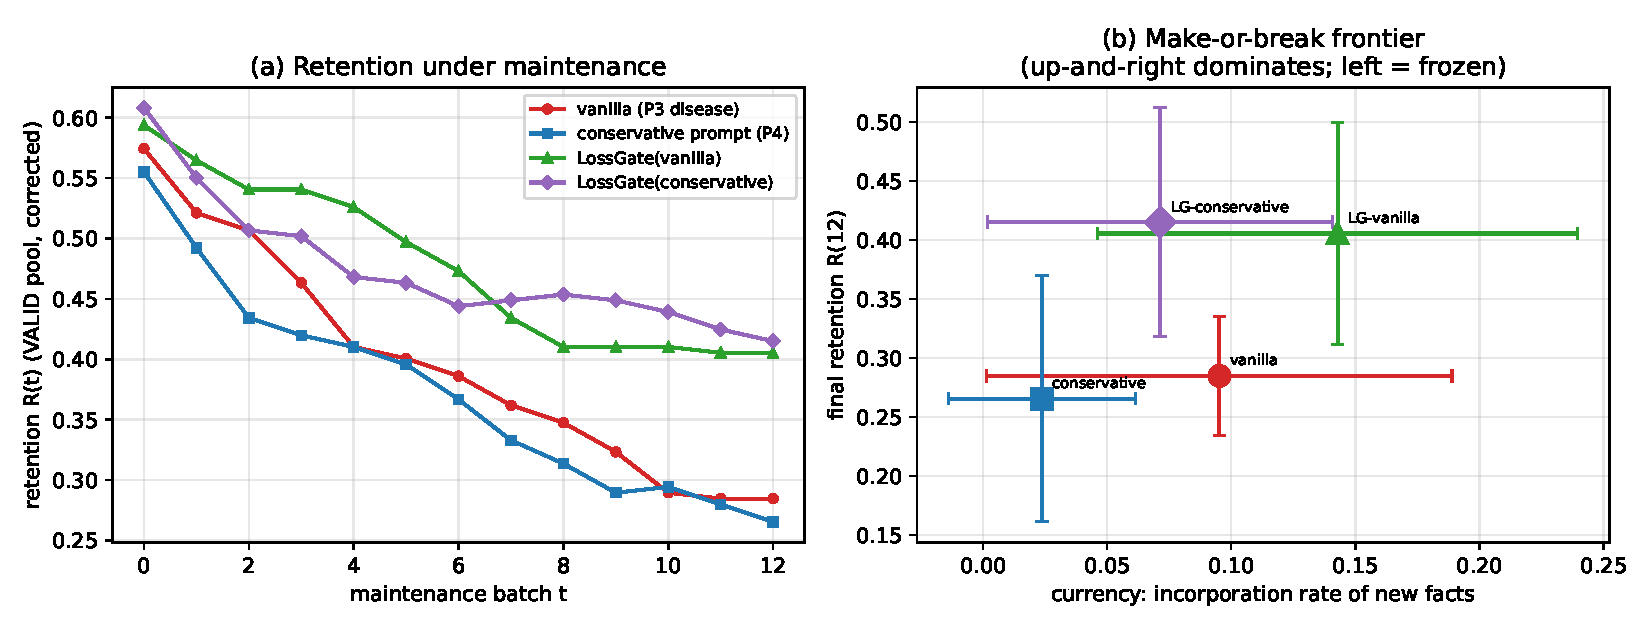
\includegraphics[width=0.48\linewidth]{figures/maintain_frontier.pdf}
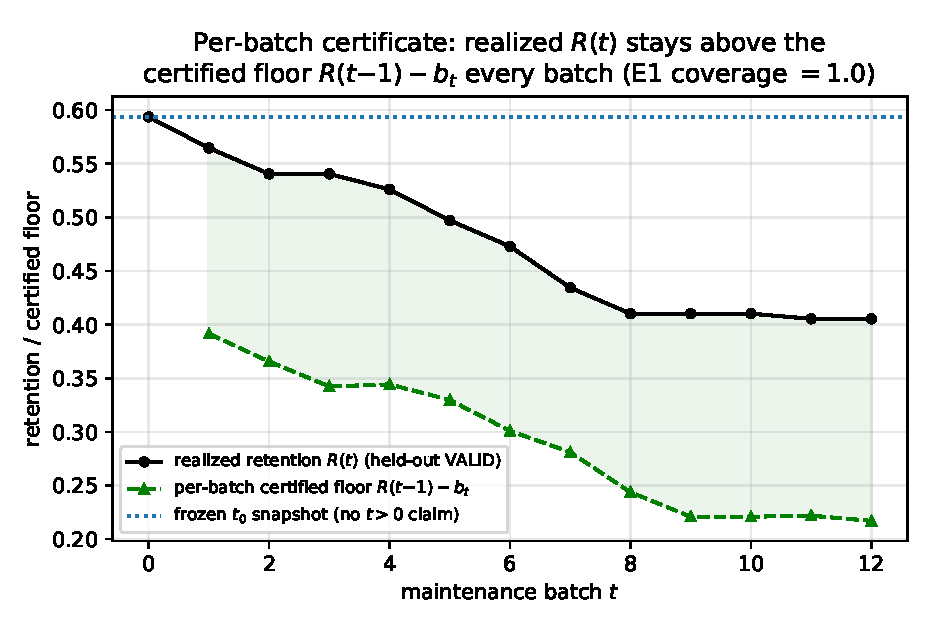
\includegraphics[width=0.48\linewidth]{figures/maintain_stream.pdf}
\caption{Left: retention vs.\ currency frontier across maintainers, gated and ungated. Right: per-batch certified floor $R(t-1) - b_t$ vs.\ realized retention $R(t)$ across the stream.}
\label{fig:lossgate}
\end{figure}

We disclose two scope limitations directly: a second model-scale run was dropped to avoid contending for shared GPUs with other running jobs, not run to completion and discarded, and it is reported as a limitation rather than silently omitted; and the LoRA-wrapped arm (gating around the trained maintainer of \S4.1 rather than a prompted one, retention lifted from $0.405$ ungated to $0.574$ gated) and the rollback-threshold ($\tau$) sweep are each single-seed and noisy, reported as directional rather than confirmed.
